% !TeX root = ../script.tex
\documentclass[../../script.tex]{subfiles}

\begin{document}
\section[Examples of the Stationary Schrödinger Equation]{Examples of the Stationary Schrödinger Equation}

We now want to solve the Schrödinger equation
\[
	\frac{-\hbar^2}{2m} \dv[2]{\psi}{x} + \epot\psi = E\psi
\]
for a few simple, one-dimensional problems. These examples will illustrate the description of classical particles as waves and the following physical consequences.

\subsection{The Free Particle}

A particle is said to be free, if it is moving in a constant potention $\phi_0$, because then $\vec{F} = -\grad{\epot}$ means that no forces are acting on the particle. 
Through a suitable choice of the zero point energy we can set $\phi_0 = 0$, i.e. $\epot = 0$, and thus get the Schrödinger equation for a free particle 
\begin{equation}\label{eq:onedschroedinger}
	\frac{-\hbar^2}{2m} \dv[2]{\psi}{x} = E\psi
\end{equation}
The total energy $E = \ekin + \epot$ is because of $\epot$ now 
\[
	E = \frac{p^2}{2m} = \frac{\hbar^2 k^2}{2m}
\]
Thus~\eqref{eq:onedschroedinger} gets reduced to 
\[
	\dv[2]{\psi}{x} = -k^2 \psi
\]
which has the general solution 
\begin{equation}\label{eq:onedsolution}
	\psi(x) = Ae^{ikx} + Be^{-ikx}
\end{equation}
The time-dependent wave function 
\begin{equation}\label{eq:onedsolutioncomplete}
	\psi(x, t) = \psi(x) \cdot e^{-i\omega t} = Ae^{i(kx - \omega t)} + Be^{-i(kx + \omega t)}
\end{equation}
represents the superposition of a planar wave travelling in the $+x$ and $-x$ direction.

The coefficients $A$ and $B$ are the amplitudes of those waves, which are determined by the boundary conditions.
For example, the wave function of electrons which are emitted from a cathode in $+x$ direction towards a detector, will have $B = 0$, since there are no particles moving in $-x$.
From this experimental setup we know that the electrons are found along the length $L$ of the path between cathode and detector. This means their wave function can only be different from zero in this region of space.
Using the normalization condition we get 
\begin{align*}
	&\int_0^L \abs{\psi(x)}^2 \dd{x} = 1 \\
	&\implies A^2 \cdot L = 1 \implies A = \frac{1}{\sqrt{L}}
\end{align*}
To determine the location of a particle at time $t$ more accurately, we will have to construct \textit{wave packets} in place of planar waves~\eqref{eq:onedsolution}
\begin{equation}
	\psi(x, t) = \int_{k_0 - \Delta k / 2}^{k_0 + \Delta k / 2} A(k) e^{i(kx - \omega t)} \dd{k}
\end{equation}
The location uncertainty of this packet at $t = 0$ is 
\[
	\Delta x \ge \frac{\hbar}{2 \Delta p_x} = \frac{1}{2\Delta k}
\]
and depends on the pulse width $\Delta p_x = \hbar \Delta k$. The larger $k$ is, the more certainly $\Delta x(t = 0)$ can be determined, but the faster the wave packet spreads.

Experimentally, this can be illustrated as follows: If we apply a short voltage pulse to the cathode at time $t = 0$, then electrons can start travelling towards the detector at this instance.
The emitted electrons have a velocity distribution $\Delta v$, such that electrons with differing velocities $v$ will not necessarily be in the same location $x$ at a later point in time $t$.
Instead they are spread over the interval $\Delta x(t) = t \cdot \Delta v$. The velocity distribution is described by $\Delta v \propto \Delta k$ of the wave packet, such that the location uncertainty $\Delta x$ 
\[
	\dv{(\Delta x(t))}{t} = \Delta v(t = 0) = \frac{\hbar}{m} \Delta k(t = 0)
\]
changes proportionally to the initial impulse uncertainty.

\subsection{Potential Step}

We are still considering the particles from the previous example, however we introduce a potential step at $x = 0$. This means we are considering the potential 
\[
	\phi(x) = \begin{cases}
		0 & x < 0 \\
		\phi_0 & x \ge 0
	\end{cases}
\]
This means the particles are still moving in direction $+x$ and are free ($\epot = 0$) if their position is $x < 0$. However at position $x = 0$ they enter into an area of higher potential $\phi(x \ge 0) = \phi_0 > 0$.
The potential energy in this area is still constant $\epot = \energy{0}$. Thus, at $x = 0$ we have a potential jump $\Delta E = \energy{0}$.
This problem has an equivalent in classic optics: a planar lightwave encountering a boundary between vacuum and material (e.g.\ a glass surface).

We divide the domain $-\infty < x < +\infty$ into two areas I and II\@. For area I with $\epot = 0$ we still have the equation~\eqref{eq:onedschroedinger} with the solution~\eqref{eq:onedsolution}
for the location part of the wave function 
\[
	\wave[I](x) = Ae^{ikx} + Be^{-ikx}
\]
where $A$ is the amplitude of the incidental wave, and $B$ the amplitude of the wave reflected from the potential step.

\textbf{Note:} The complete solution is~\eqref{eq:onedsolutioncomplete}. The temporal part of the soltuion is often omitted, because it has no influence in the stationary problems considered here.

In area II, the Schrödinger equation becomes
\begin{equation}
	\dv[2]{\psi}{x} + \frac{2m}{\hbar^2}(E - \energy{0})\psi = 0
\end{equation}
If we use the shorthand $\alpha = \sqrt{2m(\energy{0} - E)} / \hbar$ we can reduce the equation to 
\begin{equation}\label{eq:potentialstep}
	\dv[2]{\psi}{x} - \alpha^2\psi = 0
\end{equation}
This equation has the solution 
\begin{equation}\label{eq:potentialstepsolution}
	\wave[II] = Ce^{+\alpha x} + De^{-\alpha x}
\end{equation}
If 
\[
	\psi(x) = \begin{cases}
		\wave[I] & x < 0 \\
		\wave[II] & x \ge 0
	\end{cases}
\]
is a solution to the Schrödinger equation~\eqref{eq:potentialstep} on the entire domain $-\infty < x < +\infty$, then $\psi$ has to be continuously differentiable at every point,
or else the second derivative $\dd^2\psi / \dd x^2$ is not defined, and thus the Schrödinger equation is not applicable.
Using~\eqref{eq:onedsolution} and~\eqref{eq:potentialstepsolution} this results in the boundary conditions
\begin{subequations}\label{eq:boundaryconditions}
	\begin{equation}
		\begin{split}
			\wave[I](x = 0) &= \wave[II](x = 0) \\
			&\implies A + B = C + D
		\end{split}
	\end{equation}

	\begin{equation}
		\begin{split}
			\eval{\dv{\wave[I]}{x}}_0 &= \eval{\dv{\wave[II]}{x}}_0 \\
			&\implies ik(A - B) = \alpha (C - D)
		\end{split}
	\end{equation}
\end{subequations}
We can now investigate the two cases where the energy $\ekin = E$ of the incoming particle is smaller or larger than the potential step.

\subsubsection{(a) $E < \energy{0}$}
In this case, $\alpha$ is real valued and the coefficient $C$ in~\eqref{eq:potentialstepsolution} must be zero, because otherwise
\[
	\wave[II] \xrightarrow{x \rightarrow +\infty} \pm\infty
\]
If this happens, the wave function is not normalizable. With the above boundary conditions this yields
\begin{align}
	B = \frac{ik + \alpha}{ik - \alpha}A && \text{and} && D = \frac{2ik}{ik - \alpha} A
\end{align}
Thus the wave function for $x < 0$ becomes 
\begin{equation}
	\wave[I](x) = A \left[ e^{ikx} + \frac{ik + \alpha}{ik - \alpha}e^{-ikx} \right]
\end{equation}
The fraction of reflected particles is calculated as 
\begin{equation}\label{eq:reflectioncoefffirst}
	R = \frac{\abs{Be^{-ikx}}^2}{\abs{Ae^{ikx}}^2} = \frac{\abs{B}^2}{\abs{A}^2} = \abs{\frac{ik + \alpha}{ik - \alpha}}^2 = 1
\end{equation}
which means that \textit{all} particles are being reflected if $E < \energy{0}$. This corresponds to the expected classical behaviour or particles.
However there is a notable difference to classic particle mechanics:
\begin{tcolorbox}
	The particles are not being reflected at $x = 0$, but instead penetrate the domain $x > 0$ where $\epot = \energy{0} > \ekin$ before returning,
	even if their energy $\ekin < \energy{0}$ should not be enough to do so in a classical model.
\end{tcolorbox}
The probability $P(x)$ of finding a particle in $x > 0$ is 
\begin{equation}
	P(x) = \abs{\wave[II]}^2 = \abs{De^{-\alpha x}}^2 = \frac{4k^2}{\alpha^2 + k^2} \abs{A}^2 e^{-2\alpha x} = \frac{4k^2}{k_0^2} \abs{A}^2 e^{-2\alpha x}
\end{equation}
where $k_0^2 = 2m\energy{0} / \hbar^2$. After a distance $x = 1/(2\alpha)$, the penetration probability is reduced to $1/e$ of its value at $x = 0$.

We already know this result from wave optics. Even if waves are reflected totally at a boundary with refraction index $n = n' - i\kappa$, the wave penetrates the surface of the medium before returning, and the intensity
of the penetrating wave sinks to $1/e$ of its initial value after a distance $x = 1/(2k\kappa) = \lambda/(4\pi\kappa)$.
\begin{tcolorbox}
	Particles with energy $E$ can penetrate into potential areas $\energy{0} > E$ with a certain probability, even if they shouldn't be able to according to classic particle physics.
\end{tcolorbox}
Once we accept that particles are described by waves, we can come to the conclusion that particles are allowed to exist in \textit{classically forbidden} locations.

\subsubsection{(b) $E > \energy{0}$}
In this case, the kinetic energy $ekin = E$ of the incidental particle is greater than the potential jump $\energy{0}$, and in the classical model all particles would enter the area $x > 0$,
losing speed in the process, because their kinetic energy decreases to $\ekin = E - \energy{0}$. What does this look like in the wave model? The quantity $\alpha$ is now purely imaginary, so we introduce the real quantity
\begin{equation}
	k' = \frac{\sqrt{2m(E - \energy{0})}}{\hbar} = i\alpha
\end{equation}
The solution~\eqref{eq:potentialstepsolution} then becomes 
\begin{equation}
	\wave[II] = Ce^{-ik'x} + De^{ik'x}
\end{equation}
Since there are no particles moving in the $-x$ direction, we know that $C = 0$, and we are left with $\wave[II] = De^{ik'x}$.
From the boundary conditions~\eqref{eq:boundaryconditions} we can deduce 
\begin{align}
	B = \frac{k - k'}{k + k'}A && \text{and} && D = \frac{2k}{k + k'}A
\end{align}
thus leaving us with the wave functions
\begin{equation}
	\begin{split}
		\wave[I](x) &= A \cdot \left(e^{ikx} + \frac{k - k'}{k + k'} \cdot e^{-ikx} \right) \\
		\wave[II](x) &= \frac{2k}{k + k'}Ae^{ik'x}
	\end{split}
\end{equation}
The \textbf{\textit{reflection coefficient}} $R$, i.e.\ the fraction of reflected particles is then analogous to the result from optics
\begin{equation}\label{eq:reflectioncoeff}
	R = \frac{\abs{B}^2}{\abs{A}^2} = \abs{\frac{k - k'}{k + k'}}^2
\end{equation}
\textbf{Remark.} Since the wave number $k$ is proportional to the refractive index in optics ($k = n \cdot k_0$), the result~\eqref{eq:reflectioncoeff} can easily be transformed into the reflection coefficient 
\[
	R = \abs{\frac{n_1 - n_2}{n_1 + n_2}}^2
\]
of a lightwave encountering a boundary surface between two mediums with refractive indexes $n_1$ and $n_2$.

To compute the amount of particles being transmitted per unit of time (i.e.\ the number of particles passing through the area $x = x_0 > 0$ divided by the amount of particles passing through an area $x < 0$ per unit of time)
one has to consider that the velocities in both areas are different.
The ratio $v' / v = k' / k = \lambda / \lambda'$ is given by the ratio of the wave numbers. That is why the \textbf{\textit{transmission coefficient}}
\begin{equation}\label{eq:transmissioncoeff}
	T = \frac{v' \abs{D}^2}{v \abs{A}^2} = \frac{4k \cdot k'}{(k + k')^2}
\end{equation}
From comparing~\eqref{eq:reflectioncoeff} and~\eqref{eq:transmissioncoeff} we can see that 
\[
	T + R = 1	
\]
which makes sense because the amount of particles overall has to be conserved.

\textbf{\textit{Remarks.}}
\begin{itemize}
	\item Total reflection also occurs for $E = \energy{0}$. In this case $\alpha = 0$ and $k' = 0$, and thus according to~\eqref{eq:reflectioncoefffirst} or~\eqref{eq:reflectioncoeff} we see that $R = 1$
	\item Instead of a positive potential barrier one can also consider a negative one with $\energy{0} < 0$, where reflection and transmission occurs as well. 
	One has to let the wave incide from the right in order to yield the same equations. The optical equivalent would be the transition from a medium with higher optical density into one with a lower optical density.
\end{itemize}

\subsection{Quantum Tunnelling}
Now we will consider the case where the area in which the potential energy $\epot(x) = \energy{0}$ has only a finite width $\Delta x = a$,
such that for $x < 0$ and $x > a$ we have $\epot(x) = 0$, and for $0 \le x \le a$ we have $\epot(x) = \energy{0}$.

The domain is then split into three parts I, II and III, for which we repeat our previous approaches for the calculation of the wave functions 
\begin{equation}
	\begin{split}
		\wave[I] &= Ae^{ikx} + Be^{-ikx} \\
		\wave[II] &= Ce^{\alpha x} + De^{-\alpha x} \\
		\wave[III] &= A'e^{ikx}
	\end{split}
\end{equation}
We also find the boundary conditions 
\begin{align}
	\wave[I](0) &= \wave[II](0), & \wave[II](a) &= \wave[III](a) \nonumber \\
	\wave[I]'(0) &= \wave[II]'(0), & \wave[II]'(a) &= \wave[III]'(a)
\end{align}
Similar to the previous example we then find the following conditions 
\begin{align*}
	A + B &= C + D \\
	Ce^{\alpha a} + De^{-\alpha a} &= A'e^{ika} \\
	ik(A - B) &= \alpha (C - D) \\
	\alpha Ce^{\alpha a} - \alpha D e^{-\alpha a} &= ikA' e^{ika}
\end{align*}
Solving the last equation for $A'$ and inserting the relationships between $C$ and $A$ and $D$ and $A$ from the first three equations then gives us the transmission coefficient of the barrier
\begin{equation}
	^T = \frac{v \cdot \abs{A'}^2}{v \cdot \abs{A}^2}
\end{equation}

\begin{figure}
	\begin{center}
		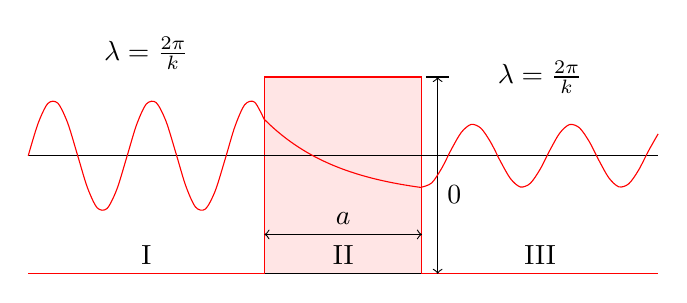
\begin{tikzpicture}
			\fill[red!10] (3, 0) rectangle (5, 2.5);
			\draw[black] (0, 0) -- node[above] {I} (3, 0) -- node[above] {II} (5, 0) -- node[above] {III} (8, 0);
			\draw[red] (0, 0) -- (3, 0) -- (3, 2.5) -- (5, 2.5) -- (5, 0) -- (8, 0);

			\draw[black] (5.05, 2.5) -- (5.35, 2.5);
			\draw[black, <->] (5.2, 0) -- node[below right] {$\energy{0}$} (5.2, 2.5);
			\draw[black, <->] (3, 0.5) -- node[above] {$a$} (5, 0.5);
		
			\draw[black] (0, 1.5) -- (8, 1.5);

			\draw[red, domain=0:3, smooth, variable=\x] plot ({\x}, {sin(5*\x r) * 0.7 + 1.5}) ;
			\draw[red, domain=3:5, smooth, variable=\x] plot ({\x}, {exp(-(\x - 3)) + 0.96});
			\draw[red, domain=5:8, smooth, variable=\x] plot ({\x}, {sin(5*(\x + 0.95) r) * 0.4 + 1.5});

			\node at (1.5, 2.8) {$\lambda = \frac{2\pi}{k}$};
			\node at (6.5, 2.5) {$\lambda = \frac{2\pi}{k}$};
		\end{tikzpicture}
	\end{center}

	\caption{Quantum tunnelling through a rectangular potential barrier}
	\label{fig:quantumtunnelling}
\end{figure}

Inserting $k = p/h$ and $E = p^2/2m$ gives
\begin{equation}
	T = \frac{1 - E/\energy{0}}{(1 - E/\energy{0}) + (\energy{0} / 4E) \cdot \sinh^2(\alpha \cdot a)}
\end{equation}
with $\alpha = \sqrt{2m(\energy{0} - E)}/\hbar$.
\end{document}